\documentclass{article}

\usepackage{listings}
\usepackage{amsmath}
\usepackage{url}
\usepackage{graphicx}

\graphicspath{}

\begin{document}


\section{Hyper parameter optimization}

The goal of hyper parameter optimization is to find the best hyperparameters for the given classifier, in order to optimise the loss function and to avoid overfitting \cite{Bergstra}. Hyperparameter optimisation is one of the most important steps in machine learning \cite{bardenet}. Some hyper parameter optimisation algorithms not only find the best hyperameters, but identify those that carry the most weight, \cite{Bergstra}.
We needed an algorithm to find the best way to tune the hyper parameters of our chosen classifiers.  As we were recommended grid search, this was the algorithm we decided to look into.  

\subsection{Grid Search}

Grid Search is an algorithm for hyperparameter optimisation. It does this by iterating over all of the variables in a given range, and selecting the best combination to use in the chosen classifier. 
As grid search was recommended to us, and is the most widely used way to optimize hyper parameters, we decided to use it in our project.

\subsection{Grid Search in Skilearn}

SkiLearn has a built in function for Grid Search \cite{gridsearch}, which is defined below:


\begin{lstlisting}
GridSearchCV(estimator, param_grid, scoring=None, fit_params=None, 
   n_jobs=1, iid=True, refit=True, cv=None, verbose=0, 
   pre_dispatch='2*n_jobs', error_score='raise',
   return_train_score=True)
\end{lstlisting}

The param \textunderscore grid is a dictionary of the parameters you want to choose and the range of parameters to try. The grid search algorithm will then run the given classifier over the entire parameter grid for the best possible combination. 

Scoring allows you to choose to train for precision or recall. Precision is the fraction of retrieved instances that are relevant, whilst recall is the fraction of relevant instances that are retrieved.

\begin{align*}
Precision &= true positive / true positive + false positive\\
Recall &= true positive / true positive + false negative 
\end{align*}

We decided to focuss on precision, as we wanted to tune accurate classifiers. 

The output of GridSearch is the a dict, with the names of the hyperparamter as keys, and the optimal result as values. 

\begin{lstlisting}

{hyperparamter: optimal value, hyperparameter: optimal value}
\end{lstlisting}

\section{Results}

The accuracy of classifiers with optimised hyperparameters were graphed against those without optimised hyperparameters:

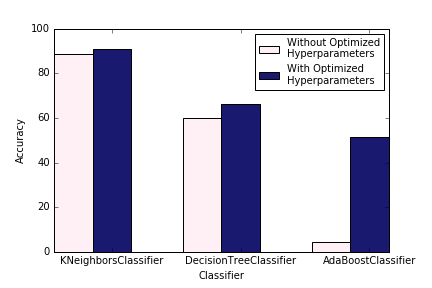
\includegraphics[scale=0.7]{acc_class}

In each of the cases, grid search clearly improved the accuracy of the classifier. This highlights the importance of hyperparameter optimisation. 

\bibliographystyle{unsrt}
\bibliography{report-references}

\end{document}

